\chapter{Contextualização da Improvisação de códigos}\label{cap:introducao}

Giovanni \citeonline[p.~117]{mori_analysing_2015} define a improvisação de códigos em relação à Música, Imagens em Movimento, Dança ou Tecelagem. É importante esclarecer que essa definição denota a aplicação em qualquer outra área, não apenas como metáfora, mas como estratégia de gerenciamento de fluxos criativos, assistido por computador:

\begin{citacao}
\traducao{\emph{Live coding} é uma técnica artística de improvisação. Pode ser empregada em muitos contextos diferentes de performance: dança, música, imagens em movimento e mesmo tecelagem. Eu concentrei minha atenção no lado musical, que parece ser o mais proeminente.}{Live coding is an improvisatory artistic technique. It can be employed in many different performative contexts: dance, music, moving images and even weaving. I have concentrated my attention on the music side, which seems to be the most prominent.}
\end{citacao}

O problema desta definição é que ela não contempla uma classe puramente técnica da improvisação de códigos, como por exemplo os registros audiovisuais de um tutorial de como escrever um aplicativo \emph{web}\disponivelem{https://www.youtube.com/watch?v=dHtyDron5ik}. No entanto, a premissa da pesquisa é, assim como Mori, situar a improvisação de códigos do ponto de vista musical. Descartamos uma discussão específica sobre imagens em movimento para evitar cair em uma digressão infinita; mas uma menção será feita em relação ao contexto musical. A discussão sobre tecelagem \ver{sec:tecelagem} contextualiza a história da computação, com suas bases conceituais do que é computação, com a prática artística investigada. Além disso, improvisadores-programadores influentes, Alex McLean, Dave Griffths (e Adrian Ward), serão apresentados. A discussão sobre Dança aprensenta a Música Eletrônica para Dançar \footnote{\cfcite{hillegonda_dj_2013}.} \ver{sec:algorave}, e a coreografia que nega o som como resultado da improvisação de códigos \ver{sec:coreografia}. Introduzindo a discussão musical \ver{sec:musica}, apresentamos alguns improvisadores brasileiros, porém nosso foco último será discutir um conjunto de regras práticas que emergiram durante uma disputa acadêmica. Isto é, a partir de uma problematização feita por \citeonline{schloss_dilemma_2003}, sobre o papel cênico (e visual) do músico que carrega um computador no palco de performance, uma resposta conjunta de McLean, Griffths, Amy Alexander, Adrian Ward, Fredrik Olofsson, Julian Rohrhuber e Nick Collins, \cite{ward_live_2004}, possibilitou a proliferação de idéias e a estruturação de um programa de investigação científica próprio para a improvisação de códigos \ver{sec:laptoptoplap}.

\section{Tecelagem}\label{sec:tecelagem}

Contextualizar a atividade têxtil é uma forma de criar uma imagem mental, de como funciona o processo de computação. Seria possível usar a imagem de um ábaco. Mas essa última imagem não considera potenciais leitores de um programa de pesquisa que inclui investigadores na área de Moda (como é o caso do Programa de Pós Graduação em Artes, Cultura e Linguagens da Universidade Federal de Juiz de Fora). Não aprofundaremos o assunto de Moda, mas sim buscamos ilustrar um código de computador. Nas palavras de \citeonline{griffths_weave2_2015},

\begin{citacao}
 \traducao{Um dos potenciais da tecelagem que eu fiquei mais interessado é a capacidade de demonstrar fundamentos de \emph{softwares} por fios -- parcialmente tornar a natureza física da computação auto-evidente, mas também como uma maneira de modelar novas formas de aprender e a entender o que são os computadores.}{One of the potentials of weaving I’m most interested in is being able to demonstrate fundamentals of software in threads – partly to make the physical nature of computation self evident, but also as a way of designing new ways of learning and understanding what computers are.}
\end{citacao}

Buscamos demonstrar na próxima seção esta natureza física da computação, para auxiliar a inclusão da tecelagem na definição de Mori.

\subsection{Charles Babbage e Joseph-Marie Jacquard}

Os computadores atuais são máquinas desenvolvidas com base no modelo teórico elaborado por Alan Turing (1912-1954). Uma representação simplista considera uma fita abstrata de tamanho variável (o quanto for necessário), dividida em células, cada uma com um alfabeto finito. Cada alfabeto possui uma quantidade de símbolos de representação finita. Um cabeçote leitor desta fita lê as instruções escritas em cada célula, e depois passa para a próxima célula. Um registrador de estados desta fita, memoriza qual foi a última operação realizada na última célula executada. Uma tabela de ações indicará novas instruções, que serão escritas nesta fita.

 Um modelo anterior ao de Turing foi elaborado por Charles Babbage (1791 -- 1871), \emph{a máquina analítica},  entre 1834 e 1836, revisado em 1837. Sua construção ocorreu após um colapso na construção de sua \emph{máquina diferencial}. O projeto não vingou, mas a partir de 1838, Babbage se envolveu com a exploração intelectual dos conceitos elaborados, para otimizar o projeto e reduzir seu custo de construção. Uma sequência de seminários em Turin (1840) resultou em uma publicação sobre a máquina analítica, em francês, escrita por um cientista italiano (L.F. Menebrea). A Condessa de Lovelace (Ada Augusta Byron King), traduziu, sob supervisão de Babbage, esta publicação para o inglês. Historicamente, os primeiros programas de computador (para serem executados na máquina analítica) foram escritos ambos por Ada e Babbage. O primeiro programa escrito era dedicado ao cálculo de uma sequência numérica conhecida como \emph{Números de Bernoulli} \footnote{Allan G. Broomley, \emph{Charles Babbage’s Analytical Engine, 1838}. Disponível em \url{http://athena.union.edu/~hemmendd/Courses/cs80/an-engine.pdf}}. Apenas uma parte da máquina foi construída antes da morte de Babbage\disponivelem{http://www.sciencemuseum.org.uk/objects/computing_and_data_processing/1878-3.aspx}.

Segundo \citeonline[p.14--21]{McLean2011}, o mecanismo do projeto de Babbage é inspirado na máquina de tear de Joseph-Marie Jacquard (1752 -- 1834). A principal contribuição da invenção, para a computação, foi um sistema que consiste em um cabeçote leitor de cartões perfurados. Na máquina de tear de Jacquard, a organização dos furos indicam, até hoje, uma rotina têxtil. Já no computador mecânico de Babbage, o cartão perfurado indicava estados binários que conduzem ao cálculo numérico:

\begin{citacao}
\traducao{A indústria têxtil vislumbrou a primeira máquina programável de ampla utilização: a cabeça de tear Jacquard, uma tecnologia ainda usada. Longas tiras de cartão são alimentados na cabeça de tear Jacquard, que lê padrões perfurados no cartão para guiar a intrincada padronização de tecidos. O cabeçote Jacquard não computa, mas foi admirado por Charles Babbage, inspirando o trabalho na sua máquina analítica mecânica, a primeira concepção de um computador universal programável. Embora Babbage não tenha obtido sucesso em construir a máquina analítica, seu projeto inclui um mecanismo de entrada de cartão similar ao cabeçote Jacquard, mas com  padrões perfurados descrevendo cálculos abstratos ao invés de fios têxteis.}{
The textile industry saw the first programmable machine to reach wide use: the head of the Jacquard loom, a technology still used today. Long strips of card are fed into the Jacquard head, which reads patterns punched into the card to guide intricate patterning of weaves. The Jacquard head does not itself compute, but was much admired by Charles Babbage, inspiring work on his mechanical analytical engine (Essinger, 2004), the first conception of a programmable universal computer. Although Babbage did not succeed in building the analytical engine, his design includes a similar card input mechanism to the Jacquard head, but with punched patterns describing abstract calculations rather than textile weaves.
}
\end{citacao}

%\begin{figure}[!h]
%  \centering
%  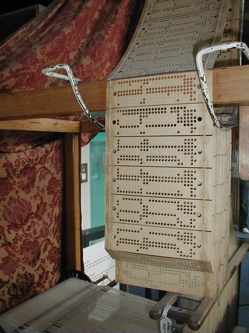
\includegraphics[scale=0.82]{imagens/Jacquard.jpg}
%  \caption{Cartões perfurados da máquina de tear Jacquard. \textbf{Fonte}: wikimedia.org }
%  \label{fig:jacquard}
%\end{figure} 

\subsection{Weavecoding}\label{sec:weavecoding}

Se até hoje o mesmo sistema de Jacquard é utilizado para materializar imagens mentais de formas geométricas, como improvisadores de códigos elaboram uma \emph{estratégia transversal} \ver{sec:tidal}, de transformar a imagem mental destas formas geométricas em códigos, e de códigos para o resultado desejado? De outra forma, como é realizada uma improvisação de códigos audio visuais, musicais e têxteis? Exemplificamos o caso com um grupo que criou o conceito \emph{weavecoding}. Sua definição será dada conforme apresentamos o grupo \emph{Weaving codes}\disponivelem{http://kairotic.org/about/}, em um encontro no espaço Foam Kernow\disponivelem{http://fo.am/kernow/}.

O grupo \emph{Weaving codes} foi formado para  a \traducao{(\ldots) investigação de padrões a partir das perspectivas de tecelagem e música, e através do desenvolvimento de uma linguagem de computador, e código para descrever a construção de tecidos}{We pursue these questions in the Weaving Codes- Coding Weaves project, by investigating patterns from the perspectives of weaving and music, and by developing a computer language and code for describing the construction of weaves}. É formado por membros da Universidades de Leeds, Nottingham Trent, Cambridge, Aberdeen, Copenhague; um museu (\emph{Albert Museum}), uma rede de laboratórios transdisciplinares (FoAM Kernow ); o Centro Dinamarquês para Pesquisa Têxtil, e Escola Robert Schumman de Música e Mídia de  Düsseldorf. 

Uma pequena digressão: dois membros deste grupo, Alex McLean e Dave Griffths, são praticantes e organizadores de improvisações de código como artistas-programadores. A principal contribuição dos autores foi uma heurística da improvisação de códigos, \emph{Lubeck04}, mais conhecido como \traducao{Mostre-nos suas telas}{Show Us Your Screens}, dentro de um manifesto publicado como \traducao{Programação de Algoritmo Ao vivo e Organização Temporária para sua Promoção}{Live Algorithm Programming and Temporary Organization for its Promotion} \cite{ward_live_2004}. Este tema será discutido adiante \ver{sec:showusyourscreens}.

Do manifesto à codificação têxtil, \citeonline{griffths_weave2_2015} apresenta um interessante exemplo. A partir de quatro tarefas fundamentais (rotinas), descritas no Exemplo \autoref{ex:weaving}, é possível elaborar um padrão como o apresentado na \autoref{fig:weaving}. A primeira rotina é \emph{repeat}, uma repetição de ações por contagem, ou laço iterativo (\emph{loop}); a segunda é \emph{twist}, ou dar a volta em determinados pontos; a terceira,  \emph{weave-forward}, tecer à frente do ponto; e a quarta, \emph{weave-back}, tecer atrás do ponto . Do lado direito da imagem (ver p.~\pageref{fig:weaving}), é simbolizado o ``código criptografado de tecido'', ou as operações fundamentais para um determinado padrão têxtil. Do lado esquerdo, seu resultado-padrão, uma textura de losangos e zigue-zagues.  

\begin{example}{Um código-fonte que gera um tecido semelhante à \autoref{fig:weaving}.}
\label{ex:weaving}

\begin{minted}[fontsize=\footnotesize]{cl}
(twist 3 4 5 14 15 16)
(weave-forward 3)
(twist 4 15)
(weave-forward 1)
(twist 4 8 11 15)

(repeat 2
 (weave-back 4)
 (twist 8 11)
 (weave-forward 2)
 (twist 9 10)
 (weave-forward 2)
 (twist 9 10)
 (weave-back 2)
 (twist 9 10)
 (weave-back 2)
 (twist 8 11)
 (weave-forward 4))
\end{minted}
\end{example}

\begin{figure}[!h]
    \centering
    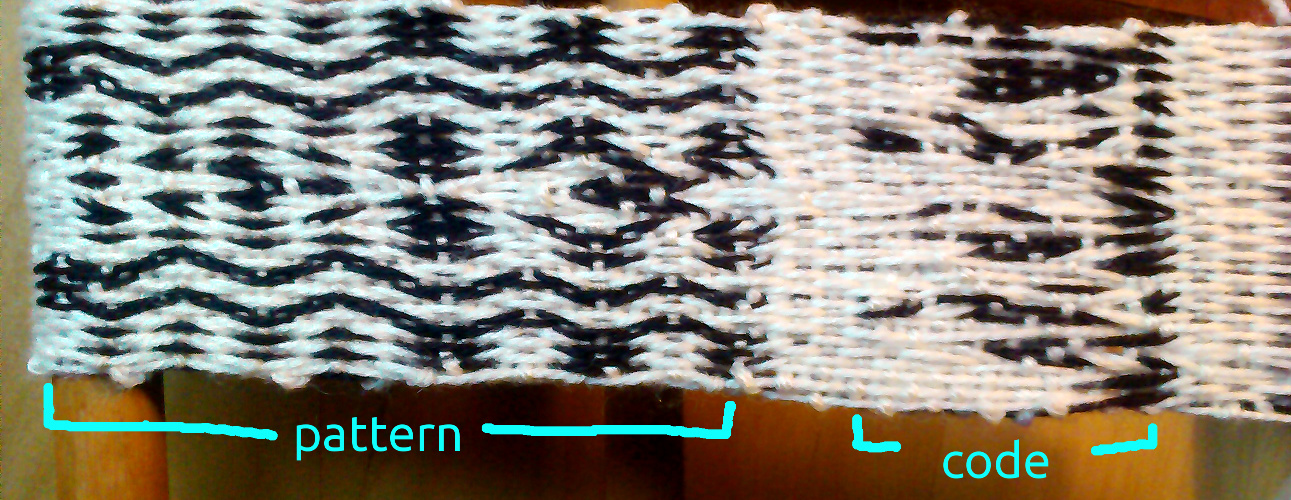
\includegraphics[scale=0.31]{imagens/weaving.jpg}
    \caption{Tecido resultante da prática \emph{Weaving code}. \textbf{Fonte}: \citeonline{griffths_weave2_2015}.}
  \label{fig:weaving}
\end{figure}

Esta experiência de \emph{weavecoding} pode ser aplicada em uma performance. Griffths ilustra uma performance arquetípica da improvisação de códigos: programadores escrevendo enquanto os resultados são projetados em superfícies planas \ver{fig:weavecoding}. A tecelagem é programada por meio de um dispositivo tangível \ver{fig:weavecoding2}, uma matriz de botões acopláveis, desenvolvida por Ellen Harlizius-Klück (investigadora da história da matemática, filosofia e tecelagem da Grécia Antiga na Universidade de Copenhague\disponivelem{http://www.saumweberei.de/}) e Alex McLean \ver{fig:weavecoding2}. Imagens em movimento foram projetadas como capturas das atividades têxteis e processadas por Griffths. 

\begin{figure}[h]
  \centering
  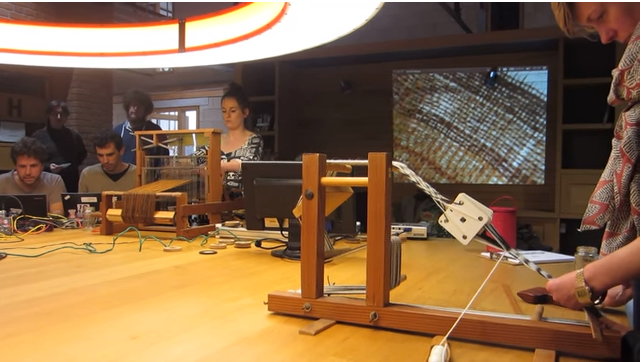
\includegraphics[scale=0.65]{imagens/weaving.png}
  \caption{Performance no Foam Kernow. \textbf{Fonte}: \citeonline{griffths_weave_2015}.}
  \label{fig:weavecoding}
\end{figure}

\begin{figure}[h]
  \centering
  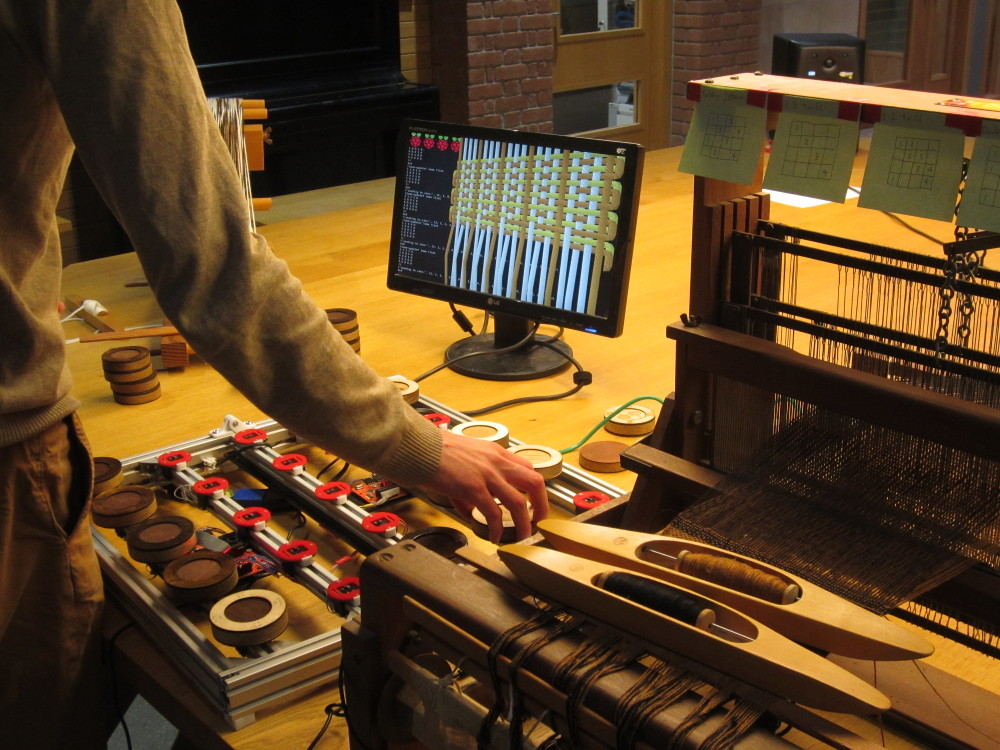
\includegraphics[scale=0.8]{imagens/weavecoding.jpg}
  \caption{ Alex McLean manipulando uma Matriz de botões para tecelagem, conectado a um Raspberry Pi. \textbf{Fonte}: \citeonline{griffths_weave_2015}.}
  \label{fig:weavecoding2}
\end{figure}

\begin{citacao}

\traducao{
Uma das idéias originais era combinar tecelagem e codificação em um cenário de atuação, ambos para fornecer uma forma de tornar a codificação ao vivo mais inclusiva com a tecelagem, e ao mesmo tempo esclarecer os processos de pensamentos digitais envolvolvidos na tecelagem (\ldots) Nossa audiência consistiu de pesquisadores de artesanato, biólogos antropológicos, arquitetos, designers de jogos e tecnólogos -- foi mais do que antecipamos! Alex e eu disponibilizamos alguns códigos de música do \emph{slub} para tecer, e minha parte favorita foi projetar a tecelagem ao vivo.
}{
One of the original ideas we had was to combine weaving and coding in a performance setting, to both provide a way to make livecoding more inclusive with weaving, and at the same time to highlight the digital thought processes involved in weaving. (\ldots) Our audience consisted of craft researchers, anthropological biologists, architects, game designers and technologists -- – so it all went on quite a lot longer than we anticipated! Alex and I provided some slub livecoded music to weave by, and my favourite part was the live weaving projection.
}
\end{citacao}

Esta descrição de Griffths possui uma documentação audiovisual \disponivelem{https://www.youtube.com/watch?v=XrnIVUp9QgM}. É interessante notar que a menção ao grupo \emph{Slub} auxilia a discussão musical, e ao mesmo tempo articula esta seção com a próxima. 

\subsubsection{Slub}

A banda \emph{Slub} começou em 2000, como uma colaboração entre Adrian Ward e Alex McLean. A premissa do duo era utilizar a atividade de programação para realização de uma Música Eletrônica de Dança\footnote{\cfcite{hillegonda_dj_2013}}. Sua primeira reunião foi em 2001, no \emph{Paradiso club} em Amsterdã, durante o festival \emph{Sonic Arts}. Em 2005 Griffths se juntou ao duo durante o festival \emph{Sonar}, o que abriu espaço para o desenvolvimento de uma estética de videogames \cite[p.~138--140]{McLean2011}.

É interessante notar que a improvisação de códigos já era mencionada em documentações de \emph{softwares}, antes do \emph{Slub} ou do manifesto de \citeonline{ward_live_2004}. No entanto, as metodologias de improvisação de códigos são diversas. A utilização de ambientes como \emph{SuperCollider}, \emph{iXiLang}, PureData ou Max/MSP, estão restritas ao contexto de linguagens de domínios específicos\footnote{\emph{Domain Specific Language} ou DSL.}. O então duo \emph{Slub} seguiu o seguinte caminho: a utilização de linguagens de propósito geral\footnote{\emph{General-Purpose Language} ou GPL.}, como Perl, REALBasic e Scheme \ver{sec:impromptu}. Além disso, uma descrição destes sistemas GPLs oferecem a descrição de uma característica interessante. Por exemplo, a justificativa de aceitação de uma música para dançar \ver{sec:algorave} é feita através de uma postura bastante trivial, projetar o que está fazendo no computador; no entanto esta trivialidade não deve ser subestimada, afinal hoje ela é considerada como uma regra heurística. Segundo \citeonline[p.~139]{McLean2011}:

\begin{citacao}
\traducao{Um sistema Slub antigo é descrito em detalhes por \citeonline{collins_generative_2003}. De maneira breve, ele apresentava um sintetizador, um antigo sistema de codificação ao vivo escrito por Ward, e uma série de programas geradores de batidas e linhas de baixo escritos por McLean. Embora o seu principal objetivo era musical, o Slub gostava de ser confrontado com o desafio de serem aceitos como programadores que fazem música. Para este fim, começou projetando suas telas de audiências com uma sobreposição conceitual, entre seu \emph{softwares} artesanais, e a música que  produziam com seu uso.}{An early Slub system is described in detail by \citeonline{collins_generative_2003}. In brief it featured a synthesiser and early live coding system written by Ward, and a Number of beat and bass-line generating programs by McLean. Although their primary aim was musical, Slub enjoyed beign faced with the challenge of beign accepted as programmers who make music. To this end they began projecting their screens audiences with the conceptual overlap between their and-crafted software and the music they produced using it.}
\end{citacao}

Em 2004, com a formação do TOPLAP \ver{sec:toplap}, Ward e McLean focaram seus eforços no desenvolvimento de ambientes de improvisação de códigos. É interessante notar que os sistemas elaborados,  são uma mistura de linguagens textuais, \emph{patching} e interfaces gráficas de usuário\footnote{\emph{Graphical User Interfaces} ou GUIs.}: \traducao{O \emph{Slub} controlava sua música usando interfaces criadas por e para eles mesmos. Eles variam desde as $[$interfaces$]$ aparentemente convencionais para as abstratas, e das  gráficas para a inteiramente textuais.}{Slub control their music using user interfaces created by and for themselves. These vary from the apparently conventional to the abstract, and from graphical to entirely textual.}
\cite[p.~323]{collins_generative_2003}. A descrição abaixo detalhada algumas das funções destes programas, bem como um processo de composição por redes que será discutido em outra oportunidade \ver{sec:baiasaofranscisco}:

\begin{citacao}
\traducao{Por detrás das interfaces \emph{slub} residem os processos 'composicionais' ou 'musicais' -- muitos pedaços de códigos separados, escritos como exploração de idéias musicais. Cada pedaço de código descreve um experimento em áreas como matemática combinatorial, progressões de acordes, modelos sonificados para as pessoas dançarem, métricas que sofrem transformações, batidas sincopadas algorítmicas, e outros. (\ldots) Estes processos composicionais enviam mensagens de um para o outro através de uma rede TCP/IP usando um protocolo de linha de comando. As mensagens viajam através de um servidor central, que administra a sincronização temporal entre os processos \emph{Slub}. (\ldots) O protocolo de rede resolve um problema que poderia, de outra forma, ser insolúvel: Adrian e Alex muitas vezes tomam abordagens muito diferentes para fazer música. Contudo eles não tem que argumentar sobre como a música é feita. Porque eles concordaram sobre, e implementaram um protocolo de rede, eles são livres para fazer música do jeito que gostarem, sabendo que seus programas irão sincronizar um com o outro.}{Behind the slub interfaces lie the ‘compositional’ or ‘musical’ processes – many separate pieces of code written as explorations of musical ideas. Each piece of code describes an experiment in such areas as combinatorial mathematics, chordal progressions, sonified models of dancing people, morphing metres, algorithmic breakbeats, and so on. (\ldots) These compositional processes send messages to one another other across a TCP/IP network using a line-based protocol. The messages travel via a central server, which also manages time sync between all the slub processes. (\ldots) The network protocol solves a problem which might otherwise be unsolvable: Adrian and Alex often take very different approaches to making music. However, they don’t have to argue about how the music is made. Because they agreed upon and implemented a network protocol between their programs, they are free to make music however they like, knowing that their programs will synchronise with each other.} 
\end{citacao}

\section{Dança}\label{sec:danca}

A Dança é ilustrada de duas maneiras. A primeira é dança como fim de uma improvisação musical. O código recodificado, e projetado de maneira semelhante ao \emph{Slub}, corre o risco de ser a atração principal. O segundo caso foge do escopo sonoro; uma coreógrafa codifica apenas a orientação espacial de uma bailarina, resultando em uma sensação de quietude sonora. É uma posição que diverge da maioria dos trabalhos apresentados, mas é pouco discutido no âmbito musical. 

\subsection{Algorave}\label{sec:algorave}

Sobre o termo \emph{algorave}, é interessante notar um comportamento criativo combinatorial \ver{sec:criatividade}. A compositora colombiana Alexandra Cárdenas, em entrevista com \citeonline{chesire_algorave_2013}, aponta que Nick Collins e Alex McLean combinaram dois termos \emph{algorithm}, e \emph{rave}, durante uma \emph{gig} (um termo utilizado no início do \emph{jazz} para caracterizar um trabalho temporário). Após sintonizarem em uma estação de rádio, decidiram cobinar a música transmitida com a programação de uma música semelhante:

\begin{citacao}
\traducao{
Algorave 'comecou como uma piada', de acordo com Alex McLean, um pesquisador de música computacional e um dos três de uma banda chamada \emph{Slub}, que têm improvisado códigos por 13 anos. Ele veio com um termo enquanto conduzia uma \emph{gig} em Nottingham com seu amigo Nick Collins (que tocava ``datapop'' sob o nome Sick Lincoln) no final de 2011. 'Nós sintonizamos em uma estação pirata tocando \emph{happy hardcore}, e nós pensamos que seria bom programar alguma música \emph{rave}.' Deste então, McLean organizou oito \emph{algoraves} informais no mundo.
}
{
Algorave "started as a joke", according to Alex McLean, a computer-music researcher and one-third of a band called Slub that's been live coding for 13 years. He came up with the term while driving to a gig in Nottingham with his friend Nick Collins (who plays "datapop" under the name Sick Lincoln) in late 2011. "We tuned into a pirate station playing happy hardcore, and we thought it would be good to program some rave music." Since then, McLean has organised eight informal algoraves around the world. 
}
\end{citacao}

Em seu artigo ``Algorave: Live Performance of Algorithmic Electronic Dance Music'', \citeonline[p.~356]{collins_algorave_2014} sustentam que as estruturas das práticas do \emph{algorave} são anteriores à improvisação de códigos, utilizadas por praticantes da Música Eletrônica para Dançar. O que mantêm a relação entre os dois é a prática de projeção do código \ver{sec:laptoptoplap}.

\begin{citacao}
\traducao{
\emph{Algorave} não é sustentado exclusivamente por \emph{live coders}, mas estes têm mantido uma forte presença em todos os eventos até agora. É assim talvez porque a tradição do \emph{live coding} de projetar telas motiva todo o esforço; onde algoritmos não estão visíveis por períodos de tempo durante uma \emph{algorave}, se corre o risco das coisas parecerem muito como um evento de música eletrônica padrão.
}
{Algorave is not exclusively a preserve of live coders, but they have maintained a strong presence at every event thus far. This is perhaps because the live coding tradition of projecting screens help motivates the whole endeavour; where algorithms are not made visible for periods during an algorave, we run the risk of things feeling much like a standard electronic music event.}

\end{citacao}

Focando em um recorte histórico da Música Eletrônica para Dançar, \citeauthoronline{collins_algorave_2014} descrevem uma sequência de eventos (desenvolvimentos de \emph{softwares} e apresentações). Em 1992, Charles Ames disponibiliza o \emph{Cybernetic Composer}, \traducao{um \emph{software} com um sistema baseado em Inteligência Artificial que compõe musica em uma variedade de estilos populares.}{an AI based software system that composes music in a variety of popular styles. Disponível em \url{http://www.kurzweilai.net/charles-ames}}. Em 1994, o duo \emph{Koan}, formado pelos DJs Daniel Roeth e William Grey, realizam adaptações para entretenimento com base no \emph{ambient music} de Brian \citeonline{eno_music_1978}. \emph{Aphex Twin} (Richard David James) cria em 1997 o termo \emph{live club algorithm}. Em 1999, o protocolo para edição audiovisual ao vivo \emph{bbcut} \cite{collins_bbcut_2003} é incluído nos \emph{opcodes} do \emph{CSound}\footnote{Disponível em \url{https://csound.github.io/}.}, e do \emph{Supercollider}\disponivelem{http://supercollider.sourceforge.net/audiocode-examples/}. Em 2000 o então duo \emph{Slub}, realizam performances, autodenominadas \emph{generative techno}, com abordagem \emph{gabba}. Em 2001 é identificada a utilização de redes neurais para composição de padrões semelhantes ao \emph{drum'n'bass}. Em 2004 é fundado o TOPLAP em uma casa noturna de Hamburgo.

Ilustramos três casos recentes, onde a improvisação de códigos é uma técnica utilizada. Junto com a improvisação de códigos, são utilizados um instrumento eletrônico, voz, e um instrumento elétrico. O inglês Canute, o mexicano Mico Rex e a colombiana residente na Alemanha, Alexandra Cárdenas.

\begin{figure}[!h]
  \centering
  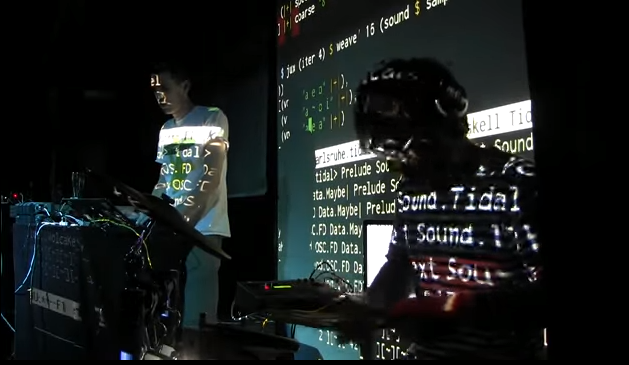
\includegraphics[scale=0.71]{imagens/canute.png}
  \caption{Performance do duo Canute (Karlesruhe, 2015) \textbf{Fonte}: \citeonline{mclean_canute_2015}.}
  \label{fig:canute}
\end{figure}

O registro audiovisual do duo Canute, Matthew Yee-King (bateria eletrônica) e Alex McLean (\emph{laptop}), reforça o arquétipo comentado anteriormente (p.~\pageref{fig:weaving}). A recomendação ``Obscurantismo é perigoso, mostre-nos suas telas''\ver{sec:showusyourscreens} é seguida à risca. Categorizações musicais como \emph{club} e \emph{chordpunch} são mencionados na descrição do vídeo. É curioso notar que, em alguns momentos do vídeo, certas modificações nos códigos causam uma perturbação brusca em sistema de ritmos, percebido através do fluxo musical. Em alguns momentos Yee-King mantem o fluxo, mas em outros o instante musical codificado leva um curto período de tempo para ser sincronizado, o que leva Yee-King a se confundir, e por um breve instante, escutar o código e aí retornar à execução. Essa quebra no fluxo musical pode atrapalhar o fluxo de movimentos do corpo. No final deste capítulo, discutimos que este pode não ser \emph{a priori} um erro do instrumentista, mas sim um problema entre o não-esforço cênico de McLean e o esforço de Yee-King. Esta questão cênica será mencionada na \autoref{sec:showusyourscreens}.

\begin{figure}[h]
  \centering
  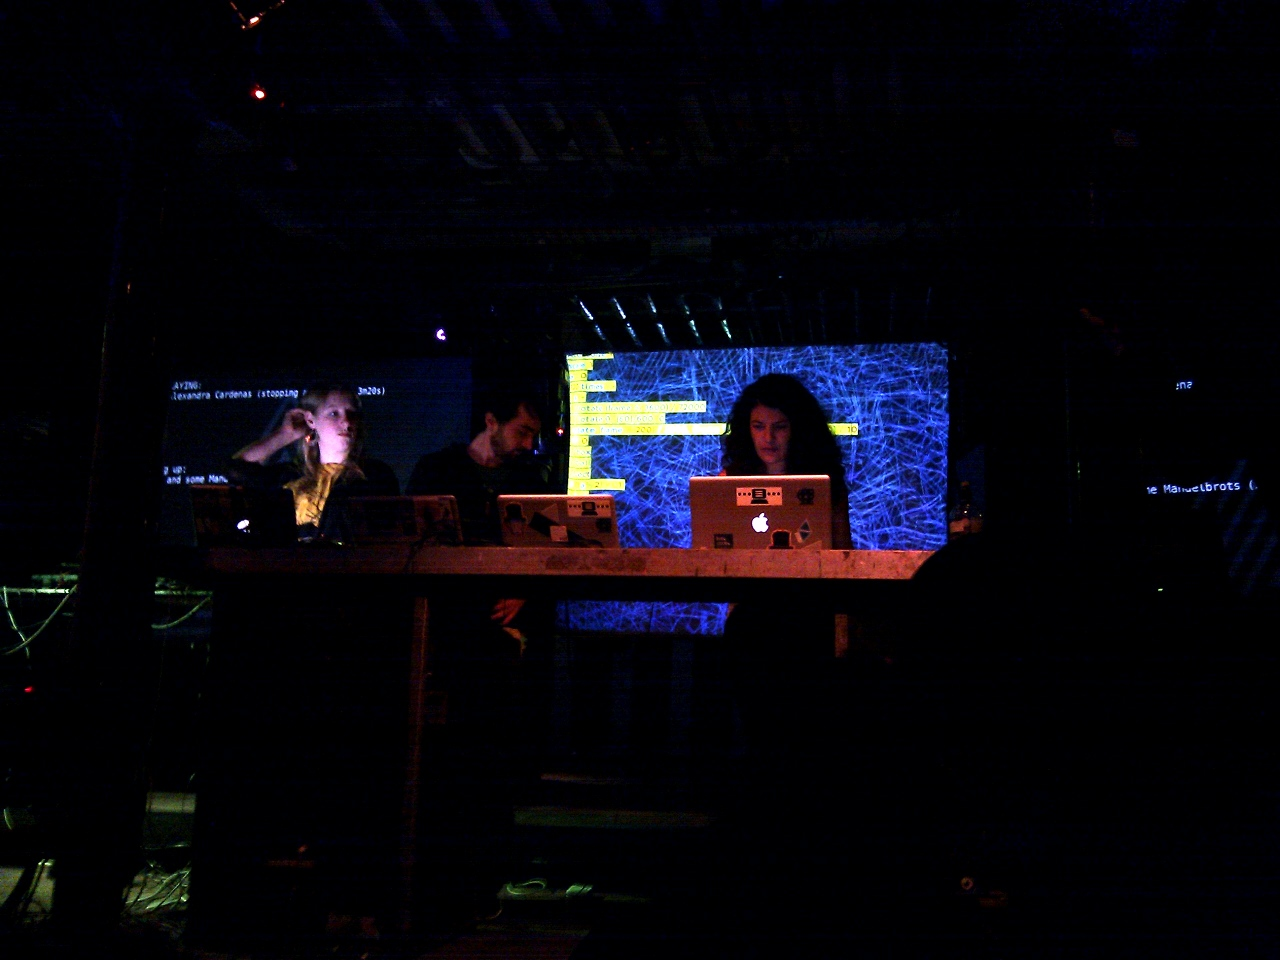
\includegraphics[scale=0.3]{imagens/cardenas.jpg}
  \caption{Performance do duo Mico Rex (Londres, 2013) \textbf{Fonte}: \citeonline{griffths_algorave_2013}.}
  \label{fig:cardenas}
\end{figure}

\begin{figure}[!h]
  \centering
  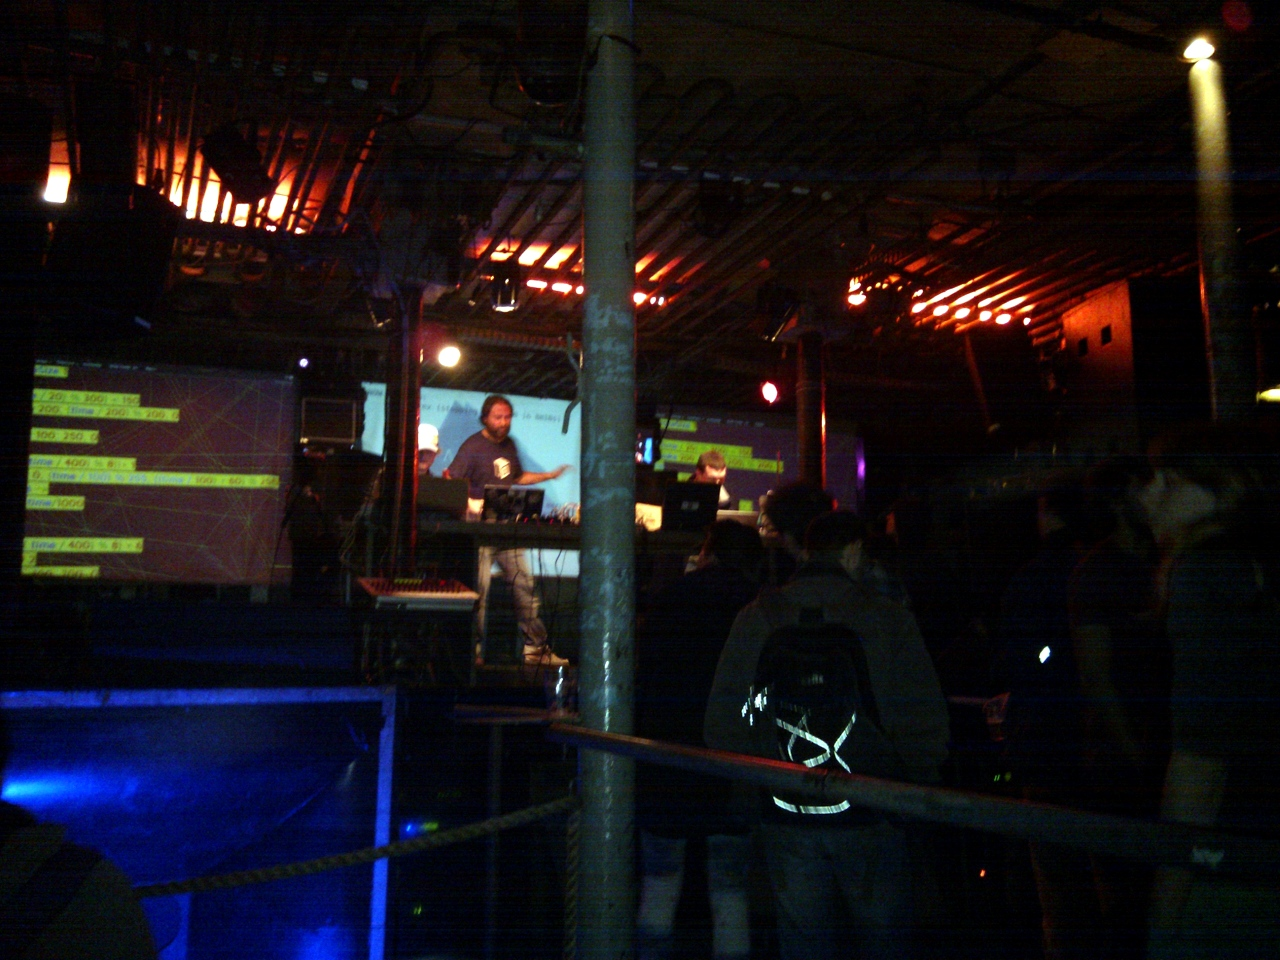
\includegraphics[scale=0.3]{imagens/algorave.jpg}
  \caption{Performance do duo Mico Rex (Londres, 2013) \textbf{Fonte}: \citeonline{griffths_algorave_2013}.}
  \label{fig:micorex}
\end{figure}

Griffiths registra uma \emph{rave} na embarcação  MS Stubnitz, em Canary Wharf, Londres, em 2013. Cárdenas e Ernesto Romero/Jorge Ramírez -- Mico Rex, \ver{fig:micorex} -- tocam neste evento. Encontramos um registro audiovisual de curta duração da apresentação do duo Mico Rex\disponivelem{https://vimeo.com/65309754}, mas não de Cárdenas. Exemplos sonoros específicos estão disponíveis nas redes sociais \emph{SoundCloud} e \emph{Vimeo} \footnote{\url{https://soundcloud.com/tiemposdelruido} e \url{https://soundcloud.com/micorex/}.}. Notas descritivas nestes perfis especificam instrumentos e linguagens de programação, mas não o processo criativo. MicoRex utiliza voz e \emph{programação} ao vivo com o ambiente de programação \emph{SuperCollider}\ver{sec:supercollider}. Entre as categorizações musicais mencionadas, \emph{electro-pop}, \emph{8bits/glitch}, \emph{electro}, \emph{punk}, \emph{bolero} e \emph{breakz}. Cárdenas realiza suas performances com guitarra e programação ao vivo com o \emph{SuperCollider}. É interessante que Cárdenas menciona a utilização de\emph{techno}, \emph{dubstep} e \emph{noise} -- além de distorções, utliliza um misto de instrumento expandido (objetos diversos jogados, friccionados, apoiados na guitarra) e retroalimentação de sinais com níveis saturados.  

\subsection{Coreografia}\label{sec:coreografia}

O segundo exemplo de um contexto de dança é projeto de Kate Sichio, \emph{Hacking the Body}/\emph{Hacking Choreography}. Dois trabalhos (\emph{Hacking Coreography} \emph{v.01} e \emph{v.02}), mais um, \emph{Hacking The Body 2.0}, serão colocados em discussão para ilustrar: \emph{i}) uma estratégia metafórica do código em uma performance de dança; \emph{ii}) uma estratégia transversal \ver{sec:tidal} de codificação de movimentos ; \emph{iii}) problematização do som ou imagem como resultado da improvisação.

Para Sichio, a relação entre a atividade de escrever programas, e a dança, é parte de um trabalho contínuo entre notação de coreografias e a improvisação de movimentos. É importante mencionar que, no escopo da pesquisa de Sichio, são raras as referências aos aspectos sonoros. Diferente das indicações estritas de um pentagrama musical, a partitura de dança ofereçe mais um guia para os movimentos do corpo. Isso significa que, do ponto de vista computacional, a partitura coreográfica é mais próxima do código escrito em uma linguagem de computador do que a partitura musical tradicional. É curioso notar que ocorre até mesmo uma assimilação do pensamento algorítmico na Dança, chamado por \citeonline[p.~31]{sichio_hacking_2004}, através de \citeonline[cap.~1, p.~3]{downie_choreography_2005}, de \emph{Sensibilidades Computacionais}. Ou dispositivos metafóricos elaborados por coreógrafos como Merce Cunningham, Trisha Brown, Bill T. Jones, e William Forsythe -- \traducao{mecanismos de generalização e abstração, representação da coreografia e dança como computação}{mechanisms of generalization and abstraction, choreography as representation, dance as computation} \cite[cap.~1, p.~2--4]{downie_choreography_2005}:

\begin{citacao}
\traducao{Esta sensibilidade computacional é presente em dois níveis em um trabalho destes coreógrafos. Primeiramente, em seus processos coreográficos -- os sistemas, métodos, e notação através dos quais os coreógrafos criam a dança. Segundo, no trabalho ele mesmo, finalizado, que aparece no palco e é interpretado pelo observador. As primeiras invenções e proclamoções de Cunningham -- a democracia do espaço do palco, e a redescoberta do que está atrás do dançarino como ponto de origem do movimento -- pode ser interpretado como generalizações do tipo; qualquer ponto do palco é a ``frente'', e conectado por um conjunto de articulações pode ser pensado como um membro. O que eram constantes, uma vez especificados em uma descrição rígida, se tornam variáveis em uma estrutura generativa.}{This computational sensibility is present at two levels in the work of these choreographers. Firstly, in their choreographic processes — the systems, methods, and notations through which the choreographers create the dance. Secondly, in the finished work itself, as it appears on stage and as it is interpreted by the viewer. (\ldots) Cunningham’s earliest inventions and proclamations — the democracy of the stage space, and the rediscovery of the dancer’s back as a point of origin of motion — can be interpreted as generalizations of a kind; any point of a stage can be a “front”, and any connected set of joints can be thought of as a limb. What were once specified constants in a rigid description become variables in in a generative framework.}
\end{citacao}

O projeto \emph{Hacking the Body}/\emph{Hacking Choreography} será descrito a partir de \emph{Hacking Choreography beta v.01}, que vai até \emph{Hacking Choreography beta v.04}, apresentados no \emph{Lincoln Performing Arts Centre} em janeiro de 2012 e o último, em maio de 2013 no \emph{Gnarl Festival} (Inglaterra).

\subsubsection{Hacking Coreography}

A experiência parte de uma primeira versão (\emph{v.01}), um \emph{hackeamento} de uma Partitura de Eventos do artista Alison Knowles (mais especificamente a peça de performance \#8, de 1965) . Por exemplo, a partitura é projetada em um espaço de performance, e dançarinos lêem a partitura (ver exemplo \ref{code:knowles}), sem ensaios prévios: 

\begin{example}{Partitura original de Alison Knowles (1965)}\label{code:knowles}
\scriptsize
Divida uma variedade de objetos em dois grupos. 
Cada grupo é rotulado com "tudo". 
Estes grupos podem incluir diversas pessoas. 
Existe uma terceira divisão do palco, objetos vazios, rotulados com "nada". 
Cada um dos objetos é "alguma coisa". 
Um executante combina e ativa os objetos das seguintes maneiras para qualquer duração desejada de tempo :

• "alguma coisa" com "tudo"

• "alguma coisa" com "nada"

• "alguma coisa" com "alguma coisa"

• "tudo" com "tudo"

• "tudo" com "nada"

• "nada" com "nada"
\end{example}

E seguem com pedaços de papéis, segundo a orientação dada por Knowles, até que executem a última instrução. No momento em que a última rotina de movimentos é executada, é esperado entrar em um laço iterativo (\emph{loop}), e repetir as instruções desde o começo. Não é o que fazem os dançarinos, sendo que assimilam o personagem do \emph{hacker}. Em outras palavras, ao completarem a partitura, são estimulados a desconstruir os rótulos uma vez organizados, e derivar novos rótulos para novas recombinações:

\begin{citacao}
\traducao{Depois que a partitura foi completada, contudo, ela foi \emph{hackeada}. Isso significa que o executante tenta de alguma forma contornar as instruções originais. Isto foi feito sem preparações prévias e a audiência assistiu isso se desdobrar enquanto era realizada. Nesta primeira performance, o papel e os rótulos foram rasgados para criar novas palavras e categorias (\ldots) Então ao invés de ``nada''$[$Nothing$]$, foram formados dois grupos, ``não''$[$No$]$ e ``coisa''$[$Thing$]$.}{After the score was completed, however, it was then hacked. This meant that the performer had to try to somehow circumvent the original instructions. This was done with no previous preparation and the audience watched this unfold as the piece was performed.In this first performance, the paper and the labels were torn up to create new words and categories (\ldots). So instead of “Nothing” there were two new groups, “No” and “Thing.”}
\end{citacao}

A segunda experiência, \emph{Hacking Coreography v.02}, é inspirada na proposta de definir termos e associar uma ordem ao termo (como no exemplo anterior). Mas dessa vez, as orientações são escritas como um híbrido de texto discursivo, legível por um executante, e de código de computador em linguagem Java. Isto é, ele não é executável por um computador para resultar em sons, mas por um humano para resultar em movimentos.

\begin{example}{Exemplo de um hackeamento de partitura de movimentos}
\begin{minted}[fontsize=\scriptsize]{java}
/Dance/
set up()
{
dance a centre, right
dance b centre, left
}

movement()
{
move1 (dance a = rotate) (dance b = jump)
move2 (dance a = brush) (dance b = lie down)
move3 (dance a = push) (dance b = run)
move4 (dance a = step) (dance b = kneel)
}

coreography()
{
if (dancer a = rotate right 180)
then both jump = 2 feet to 1
if (dancer b = travels)
then brush = right foot
}

run(){
move1
move4
move4
move1
move2
move3
move1
move2
move3
move4
}

/hack/
{
if (dancer a = kneel)
dancer a = kneel
if (dancer a = rotate)
dancer b = rotate opposite direction 
}
\end{minted}
\end{example}

Algumas seções são apresentadas como \emph{funções} (\emph{set up, movement, coreography \emph{e} run}). A função \emph{set up} define as posições iniciais de cada ator; \emph{movement} define os tipos de movimentos que serão executados por intérpretes; \emph{coreography} define uma estrutura de fluxo destes movimentos; e por último, uma ordem de execuções é estruturada em \emph{run}. É interessante notar que Sichio aponta para um outro \emph{hackeamento} da partitura. A utilização de números, como por exemplo na função \emph{coreography}, dificultou a leitura dos intérpretes durante ensaios. Uma alteração na função \emph{coreography}, notificada abaixo da linha \verb|/hack/|, foi feita pelos próprios intérpretes para alterar a notação numérica por uma descrição textual da ação. Isso tornou o código mais legível para humanos durante a execução de movimentos. 

\subsubsection{Hacking the Body}

O \emph{Hacking The Body 2.0}, ou \emph{HTB2.0} (2015)\disponivelem{https://www.youtube.com/watch?v=iOAffWTBVE0} é uma performance mais formal. Se caracteriza por uma apresentação em um evento internacional, com um o palco-arena que reforça a hierarquia ator-público (o palco fica aproximadamente na linha da cabeça do espectador). A coreógrafa está sentada ao lado direito do palco, visível, mas debaixo de uma penumbra. Já a dançarina, cuja vestimenta branca equilibra com uma iluminação frontal e estática, expressa uma face de seriedade\ver{fig:iclcdanca}. A coreografia segue uma partitura de movimentos corporais.  Mas esta partitura não é visual (o registro não é feito em papel), o resultado da apresentação não são movimentos corporais pré-definidos, e tão pouco existe um acompanhamento musical. Esta partitura é um correlato acústico do tato, codificada por uma coreógrafa. Afastada de uma bailarina, controla a direção dos movimentos corpóreos da performance:

\begin{citacao}
\traducao{Esta peça é uma exploração de eletrônica codificada ao vivo e movimentos improvisados. Uma dançarina veste uma peça de atuadores hápticos. Estes atuadores são programados em tempo-real via OSC\footnote{N.A.: ``\emph{Open Sound Control} é um protocolo de comunicação entre computadores, sintetizadores sonoros e outros dispositivos multimídia que são otimizados para as modernas tecnologias de rede''. Disponível em \url{http://opensoundcontrol.org/introduction-osc}} para 'zunir' sobre os lados direito e esquerdo da dançarina para indicar qual lado do corpo a dançarina deve mover. A partitura é codificada ao vivo pela coreógrafa enquanto a dançarina responde por uma retroalimentação háptica. Esta peça explora o \emph{live coding} de corpos, e movimento como saída, ao invés de saídas sonoras ou visuais como encontrado em muitas execuções de \emph{live coding}
}{
This dance piece is an exploration of live coded electronics and improvisational movement. A dancer wears a custom garment of haptic actuators. These actuators are programmed real-time via OSC to 'buzz' on the right and left sides of the dancer to indicate which side of the body the dancer will move. The score is being live coded by choreographer while the dancer is responding to the haptic feedback. This piece explores live coding of bodies and movement as output rather than a sonic or visual output as found in many live coding performances. \emph{Disponivel em \url{http://iclc.livecodenetwork.org/performances.html}}.
}
\end{citacao}

\begin{figure}[!h]
  \centering
  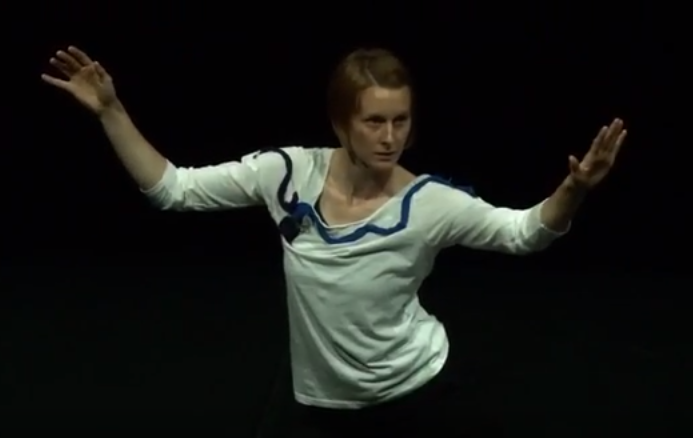
\includegraphics[scale=0.6]{imagens/iclcdanca.png}
  \caption{Dançarina (anônima) controlada por Kate Sicchio (2015) através de uma codificação improvisada. \textbf{Fonte}: \url{https://www.youtube.com/watch?v=uAq4BAbvRS4}.}
  \label{fig:iclcdanca}
\end{figure}

É interessante notar uma sensação de quietude sonora \footnote{\cfcite{koellreutter_wu-li:_1990,el_haouli_abertura_2011}}na performance, mas pouco discutida do ponto de vista musical. Como aponta a própria coreógrafa, a maioria das performances de improviso de códigos segue o seguinte procedimento: o código é criado, e um som, uma nota, uma imagem ou um vídeo são gerados, combinados, transformados de maneira contínua. Mas o padrão é a realização audiovisual. Mesmo em algumas performances de dança pesquisadas (e que não foram mencionadas neste documento), a dança e a projeção audiovisual se suportam. A criatividade deste trabalho toca um conceito técnico fundamental da computação: qual é o \emph{dispositivo de entrada e de saída} praticado nas improvisações de códigos? Sicchio responde que o corpo já é um dispositivo de entrada e saída de interações sociais e pode ser controlado por outro humano através de comandos de rede. A sensação de quietude é presente não por questões musicais, mas é definido por uma prática de dança.


\section{Música Computacional na improvisação de códigos}\label{sec:musica}

Apresentamos três exemplos de pesquisadores brasileiros. O primeiro é uma nota sobre aquilo que consideramos como as primeiras manifestações de improvisação de códigos, em 2011, coerentes com algumas regras de performance e categorizações musicais  descritas por \citeonline[ver \protect\autoref{sec:foobarbaz}, p.~\protect\pageref{sec:foobarbaz}]{ward_live_2004}. O segundo é um exemplo que apresenta uma \traducao{(\ldots) performance de \emph{livecoding} arquetípica $[$que$]$ envolve programadores escrevendo códigos no palco, com suas telas projetadas para a audiência.}{The archetypal live coding performance involves programmers writing code on stage, with their screens projected for an audience.}\cite[p.~1, ver \protect\autoref{sec:concerto}, p.~\protect\pageref{sec:concerto}]{mclean_tidal_2010}. O terceiro apresenta uma abordagem virtual, isto é, uma improvisação de códigos realizada em locais diferentes, com computadores diferentes, através de uma conexão de \emph{internet} \ver{sec:telepresenca}.  


\subsection{FooBarBaz}\label{sec:foobarbaz}

FooBarBaz é um grupo de improvisação de códigos formado por Gilson Beck, Renato Fabbri, Ricardo Fabbri e Vilson Vieira. Sua primeira apresentação foi durante o Festival Contato 2011. Os membros são ativos em um laboratório virtual conhecido como \emph{labMacambira}\disponivelem{http://labmacambira.sourceforge.net/}. Além de cientistas, participam \emph{hackativistas}, ex-programadores do Google, músicos e artistas plásticos interessados em processos criativos com assistência computacional. É interessante notar que as atividades do FooBarBaz estão sincronizadas com algumas das ideologias da improvisação de códigos, com base em regras práticas \ver{sec:showusyourscreens}. Outro ponto interessante deste grupo foi a elaboração de um manifesto próprio, chamado de \emph{Manifesto Freakcoding}, que inclue, como parte executável do manifesto, um ambiente de programação audiovisual chamado \emph{Vivace} \cite{vieira_vivace:_2015}.
 
\begin{figure}[!h]
  \centering
  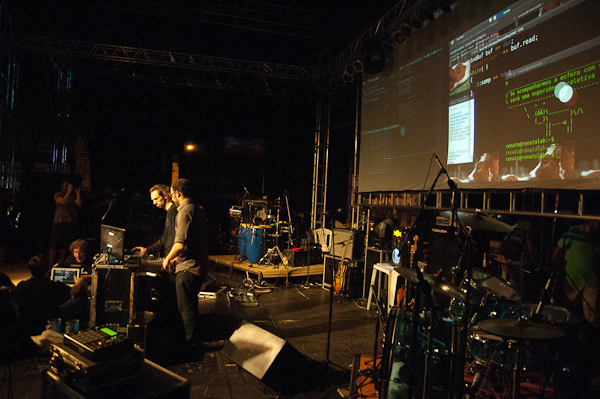
\includegraphics[scale=0.71]{imagens/Foobarbaz1.jpg}
  \caption{Festival Contato, 2011. \textbf{Fonte}: \citeonline{fabbri_wiki_2011}.}
  \label{fig:foobarbaz}
\end{figure}

Enumeramos três características que permearam as atividades do grupo, como FooBarBaz, e que ainda permeiam o contexto do \emph{labMacambira}: \emph{i}) abordagem ecosistêmica, ou diversidade de \emph{softwares}; \emph{ii}) atividade de escrita o mais simples possível; \emph{iii}) codificação como processo psico-social -- humor, como a inclusão da figura da vaca, através do programa \emph{cowsay} (``uma vaca falante configurável''\disponivelem{http://www.nog.net/~tony/warez/}), e de fotos de vacas, e REM \ver{fig:foobarbaz}. 

O membros do grupo FooBarBaz descrevem 3 dias de improvisações no Festival Contato, com a utilização de dois ambientes/linguagens de programação musical (ChucK e PD), uma linguagem de propósito geral (Python), uma ferramenta de linha de comando (C) e dois diferentes editores de texto (Emacs e Vim). Focando na improvisação de códigos com o ChucK (ver, exemplo \ref{cod:lookup}), é possível notar uma prática de improviso enraizada no sequenciamento de propriedades de uma amostra sonora, através da manipulação de listas. O escopo de cada lista, definido pelos colchetes $[$ e $]$, podem conter informações como o nome arquivo de áudio utilizado, e numericamente, sequências das posição de um \emph{sample} da amostra sonora total, dos parâmetros de diferentes taxas de amostragem, de diferentes durações da amostra, e de diferentes níveis de ganho. 

\begin{example}{Arquivo \emph{foo.ck}.}\label{cod:lookup}
\begin{minted}[fontsize=\scriptsize]{c}
["samples/fx/s20.wav"] @=> Foo.name;
[0.] @=> Foo.prop;
[.25, .15] @=> Foo.rate;
[2., 1., 1., 4.] @=> Foo.du;
[.8] @=> Foo.gain;
\end{minted}
\end{example}

O funcionamento aparentemente simplista deste código é possível através do carregamento de outros dois códigos, sendo que o primeiro depende do segundo, um código elaborado por Graham Coleman\disponivelem{http://www.dtic.upf.edu/~gcoleman/}, que estrutura uma \emph{grade temporal} (TimeGrid).

\begin{example}{Arquivo \emph{tg.ck}.}\label{cod:tg}
\begin{minted}[fontsize=\scriptsize]{c}
//basic timing operations abbreviated

public class TimeGrid {

    dur beat;
    dur meas;
    dur sect;

    int nbeat;
    int nmeas;

    //phase and magnitude of offset
    float measPhase;
    dur measOffset;
    ...

    //sync to beat
    fun void sync() {
        beat - (now % beat) => now;
    }

    fun void sync(dur T) {
        T - (now % T) => now;
    }

    //how long to sync to this duration
    fun dur syncDur(dur T) {
	return (T - (now % T));
    }

    //minimum time
    fun dur tmin(dur a, dur b) {
	return (a < b) ? a : b;
    }
    ...
}
\end{minted}  
\end{example}

Esta grade temporal é uma instância, ou seja, é possível criar diferentes grades temporais. Cada uma delas memoriza o fluxo temporal através de propriedades, tais a posição de uma unidade de tempo (\emph{beat}), compasso (\emph{meas}) e seção (\emph{sect}), e deslocamentos temporais (\emph{measPhase}, \emph{measOffset}). Existe também um mecanismo de sincronização (\emph{sync}, \emph{tmin}), o que caracteriza o conceito de níveis métricos da amostra sonora processada

\subsection{Música de concerto e imagens em movimento}\label{sec:concerto}

A performance \emph{screenBashing} de Magno Caliman (ver \autoref{fig:screenbashing}) foi realizado durante o XIII ENCUN\footnote{Encontro Nacional de Compositores Universitários em Campinas-SP no ano de 2015.}. A performance consiste no seguinte: Caliman senta-se ao computador, lateralmente à tela de projeção, com uma iluminação de penumbra. O projetor expõe o estado atual de seu \emph{laptop}, que apresenta um editor de texto. O executante começa a programar em linguagem C (ver exemplo abaixo). Um pequeno laço iterativo (\emph{for loop}) repete caracteres diversos, improvisados. Assim que termina de escrever, abre um console (ou terminal nos sistemas operacionais Unix) e compila o programa -- a compilação é um processo no qual a representação textual humana, definida pela ANSI\disponivelem{http://www.ansi.org/}, é convertida códigos binários. Este processo não demora, e o programa é executado. O resultado é uma sequência de caracteres de texto como texturas visuais. É importante lembrar que Caliman utiliza um recurso técnico do sistema operacional, que torna o terminal semi-transparente, o que permite sobreposições de texturas. A transformação da textura visual é levada a cabo através da modificação do argumento de entrada da função \verb|printf| (ver exemplo \ref{ex:magno}, p.~\pageref{ex:magno}). Esse processo ocorre com uma sensação de quietude sonora (ainda assim, este aspecto não é explorado musicalmente, mas essa não é a intenção da música). O improvisador abre códigos preparados no ambiente de programação  \emph{SuperCollider}\disponivelem{https://supercollider.github.io}, que realiza a síntese de texturas sonoras ruidosas. Segundo o compositor, foram \emph{tweets} encontrado na \emph{internet}\disponivelem{https://twitter.com/sc140tweets}. Um novo som ruidoso é adicionado para cada nova textura visual. Este processo, de alternar a codificação da textura visual, e depois executar um programa no \emph{SuperCollider}, é repetido até o fim da peça. A acumulação de sons e caracteres em movimento cria um contínuo audiovisual que, em um momento, as texturas visuais e sonoras se tornam um mesmo objeto audiovisual. Porém esta massa audiovisual sacrifica a memória RAM do computador. No auge de saturação audiovisual, a improvisação finaliza com um silêncio brusco, decorrente do congelamento do sistema operacional.


Nesta performance, a tradução ``improviso de códigos'' como correlato de \emph{livecoding} \ver{cap:introducao} se torna problemática. Segundo o próprio compositor en comunicação pessoal:

\begin{citacao}
Não acho totalmente adequado considerar como puramente um improviso. Existe, desde a concepção da peça, uma intenção de composição ali. Composição no sentido de agenciamento de materiais \emph{a priori}, entende? Claro, existe um nível de abertura ali com relação a, por exemplo, os caracteres que eu uso no loop, ou nos valores dos parâmetros do \emph{Supercollider} (\ldots). Existem sessões formais ali que, se eu tocar a peça novamente, vão se manter. Daí vc já percebe uma determinação no âmbito macro da coisa também. Em uma situação limite, eu consigo imaginar até uma partitura (de execução) para essa peça, que permitiria que outra pessoa tocasse, sem ver o video da minha performance, e chegasse em resultados bastante similares. Então eu vejo uma série de características aí que diferem de um improviso, onde se espera que uma parte grande do processo de tomada de decisão seja feita no momento da performance. Claro que essa distinção entre composição/peça/determinação e performance/improviso/indeterminação é complexa e a discussão foge totalmente do escopo do seu trabalho. Mas só para atentar para esse detalhe. acredito que se imaginarmos um \emph{continuum}, uma linha onde de um lado vc tem uma improvisação totalmente livre (impossível de se alcançar, claro) e do outro uma composição 100\% determinada (tão impossível quanto), acredito que \emph{screenBashing} está posicionada mais à direita...
\end{citacao}

\begin{figure}[!h]
  \centering
  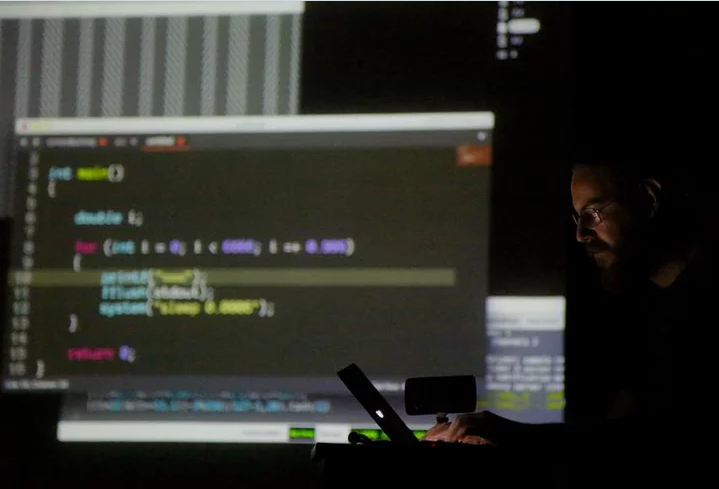
\includegraphics[scale=0.5]{imagens/screenbashing.png}
  \caption{Performance de \emph{screenBashing}. \textbf{Fonte}: \url{https://vimeo.com/148626379}.}
  \label{fig:screenbashing}
\end{figure}

O código sonoro foi pouco exposto, o que dificulta uma análise pormenorizada. Com uma valorização no aspecto imagético, para o público, é possível realizar análise do algoritmo visual, não para indicar a técnica, mas apontar a presença de uma ideologia. Limitamo-nos a comentar que o valor adicionado entre imagens em movimento, e sons, é contraposta à declaração do compositor. Por exemplo, a repetição dos algarismos seis e nove como uma menção direta (e espelhada) de signos do \emph{black metal} abstrato. Ou seja, como ouvinte e espectador, ocorreu um processo sincrético entre a imagem, o código (que de certa forma, faz parte da imagem) e o som ruidoso. No entanto o compositor declara que esta foi uma decisão tomada na hora, como uma piada, embora tenha alguma relação. Mas isso não quer dizer que, para o compositor, a sonoridade se configura como \emph{black metal}. É possível discutir se este tema ultrapassa questões de gosto ou prática sonora; ou seja, uma análise mais ampla de categorizações do gosto musical seria necessária \footnote{\cfcite{janotti_jr._a_2003,sa_se_2009}}. Por outro lado, uma segunda notação \ver{sec:imagem_mental} mais enxuta e sem erros, permite apontar a questão:

\begin{example}{Algoritmo inicial de Magno calimann}
\begin{minted}[fontsize=\scriptsize]{c}
# include <stdio.h>

int main()
{
  double i;
  
  for (int i=0; i<; i < 6666; i=+0.999)
  {
      printf("\\\\    //  \\");
      fflush(stdout)
      system("sleep 0.0006")
  }
}
\end{minted}

Execução:

\begin{minted}[fontsize=\scriptsize]{bash}
# gcc - compilador
# a.c - arquivo em linguagem c
# -o  - escreve o resultado em um outro arquivo
# a   - arquivo binario alvo
gcc a.c -o a
\end{minted}

Este código gera algumas mensagens classificadas como \emph{warnings}, ou erros de lógica, que não atrapalhou na execução deste programa. Um conflito entre números de ponto flutuante (\emph{float}) e números inteiros (\emph{int}) é parcialmente ignorado pelo compilador do computador de Caliman:

\begin{minted}[fontsize=\scriptsize]{bash}
magno.c: In function 'main':
magno.c:7:12: error: conflicting types for 'i'
\end{minted}

Resultado:

\begin{minted}[fontsize=\scriptsize]{bash}
\\\\    //  \\\\\\    //  \\\\\\    //  \\\\\\    //  \\\\\\    //
  \\\\\\    //  \\\\\\    //  \\\\\\    //  \\\\\\    //  \\\\\\  
  //  \\\\\\    //  \\\\\\    //  \\\\\\    //  \\\\\\    //  \\\\
\\    //  \\\\\\    //  \\\\\\    //  \\\\\\    //  \\\\\\    //  
\\\\\\    //  \\\\\\    //  \\\\\\    //  \\\\\\    //  \\\\\\    
//  \\\\\\    //  \\\\\\    //  \\\\\\    //  \\\\\\    //  \\\\\\
    //  \\\\\\    //  \\\\\\    //  \\\\\\    //  \\\\\\    //  \\\
\\\    //  \\\\\\    //  \\\\\\    //  \\\\\\    //  \\\\\\    //  
\\\\\\    //  \\\\\\    //  \\\\\\    //  \\\\\\    //  \\\\\\    /
/  \\\\\\    //  \\\\\\    //  \\\\\\    //  \\\\\\    //  \\\\\\  
  //  \\\\\\    //  \\\\\\    //  \\\\\\    //  \\\\\\    //  \\\\\
\    //  \\\\\\    //  \\\\\\    //  \\\\\\    //  \\\\\\    //  \\
\\\\    //  \\\\\\    //  \\\\\\    //  \\\\\\    //  \\\\\    /
\end{minted}

Correção para o algoritmo de Magno. Os novos caracteres foram inseridos por Caliman em 2$'$18$''$:

\begin{minted}[fontsize=\scriptsize]{c}
# include <stdio.h>
int main(){
  int i=0;
  for (;;i++){
      printf("=====  ______");
      fflush(stdout);
      // 30 frames por segundo (1/30)
      system("sleep 0.033");
      // 3 frames por segundo (1/3)
      // system("sleep 0.33")
  }
}
\end{minted}

Resultado:

\begin{minted}[fontsize=\scriptsize]{bash}
=====  ______=====  ______=====  ______=====  ______=====  ______=====
  ______=====  ______=====  ______=====  ______=====  ______=====  ___
___=====  ______=====  ______=====  ______=====  ______=====  ______==
===  ______=====  ______=====  ______=====  ______=====  ______=====  
______=====  ______=====  ______=====  ______=====  ______=====  _____
_=====  ______=====  ______=====  ______=====  ______=====  ______====
=  ______=====  ______=====  ______=====  ______=====  ______=====  __
____=====  ______=====  ______=====  ______=====  ______=====  ______=

\end{minted}
\end{example}

\subsection{Telepresença e espaços virtuais}\label{sec:telepresenca}

Uma performance virtual de \emph{live coding} é aquela em que dois ou mais executantes, em endereços diferentes de uma rede de computadores. Isso situa três casos, do qual especificaremos um: i) uma rede local, com computadores diferentes, mas com os improvisadores fisicamente próximos; ii) uma rede remota, privada, que comunica um conjunto de pessoas fisicamente distantes; iii) a rede mundial de computadores, onde o navegador se torna o ambiente virtual de criação musical \cite{roberts_web_2013}. Nos três casos, a premissa é compartilhar o mesmo código entre improvisadores-programadores. Podem também compartilhar do mesmo som, mas isso depende de implementações técnicas . 

O primeiro caso é bastante documentado nas \emph{live coding sessions}, sessões de improvisações que ocorrem em encontros, simpósios e \emph{workshops}, ricamente documentadas\disponivelem{https://supercollider.github.io/archive}. Um exemplo do segundo caso é descrito por \citeonline[p.~152--153]{junior_supercopair_2015}. Uma performance telepresencial em 2014, por Ben Swift, Henry Gardner e Andrew Sorensen, realizada \traducao{entre dois intérpretes-programadores localizados na Alemanha e Estados Unidos usando um servidor SSH localizado na Australia}{between two live coders located in Germany and United States using an SSH server located in Australia.}. \citeauthoronline{junior_supercopair_2015} ainda descrevem o desenvilesforço de um ambiente chamado \emph{Supercopair}\disponivelem{https://github.com/deusanyjunior/atom-supercopair}, um ambiente cooperativo de improvisação de códigos, possível através de serviços de computação em nuvem.    

Execuções remotas assíncronas (isto é, entre duas ou mais pessoas, em tempos diferentes) estão sendo exploradas a partir do uso musical de um navegador de \emph{internet}. São realizadas em \emph{apps} como \emph{Gibber} \cite{roberts_gibber:_2012}\disponivelem{http://gibber.mat.ucsb.edu/}, \emph{Wavepot}\disponivelem{http://www.wavepot.com} e \emph{Vivace} \cite{vieira_vivace:_2015}, através da biblioteca \emph{WebAudio API}\disponivelem{https://dvcs.w3.org/hg/audio/raw-file/tip/webaudio/specification.html}. Um \emph{software} na mesma direção foi desenvolvido, uma colaboração entre o autor deste documento e um membro da banca\footnote{\cfcite{lunhani_termpot_2015}}.  



\section{Discussão}

Neste capítulo delimitamos a discussão musical afim de ilustrar a improvisação de códigos do ponto de vista de uma bricolagem conceitual. Exemplificamos a prática de improvisar códigos em situações onde é possível seguir dois caminhos para criar artefatos artísticos: o primeiro segue a trilha do formalismo, com concertos, espetáculos em teatros. O segundo ocorre informalmente, e geralmente está ligado à diversão, ou um encontro como uma oficina. Por outro lado, esta divisão binária pode expandir para áreas como tecelagem, dança e música. Não discutimos a situação audiovisual em seus detalhes, pois é um campo tão particular quanto a música. No Próximo capítulo, discutiremos alguns fundamentos daquilo que foi chamado pela comunidade de improvisadores-programadores (\emph{live-coders} audiovisuais de um Norte Global) por uma proto-história da improvisação de códigos (codificação ao vivo, ou \emph{live coding}). 
